\notechapter{N-20261017}{How Should a Neural Network Take a Step? Muon and Matrix Geometry}

A neural network has millions or billions of numbers to adjust.  It is tempting to think that an optimizer merely decides how far to move each one.  But those numbers do not live in isolation.  Many form matrices, and a matrix acts on an entire space of activations.  The question of how large an update is already has several quite different answers.

This becomes particularly vivid when we compare AdamW and Muon.  Muon keeps only a momentum state for the hidden weight matrices it handles, often makes rapid progress early in language-model pretraining, and yet does not always produce a substantially better model at the end.  The practical gain may be enough to prefer it.  The mathematical puzzle is more interesting: \emph{what aspect of the geometry of a neural network does Muon manage to respect?}

We will begin with two numbers, pass through matrix duality and the polar decomposition, and then return to the whole Transformer.  Throughout, a good update is good \emph{relative to a specified norm, local objective, and budget}.  Choosing those three ingredients is precisely the difficulty.\footnote{For the algorithms and scaling observations, see Keller Jordan and collaborators, \href{https://kellerjordan.github.io/posts/muon/}{\emph{Muon: An optimizer for hidden layers in neural networks}} (2024), and Jingyuan Liu and collaborators, \href{https://arxiv.org/abs/2502.16982}{\emph{Muon is Scalable for LLM Training}} (2025).  The sources describe related but distinct practical recipes.}

\section{Two directions hidden in a tiny gradient}

Suppose the gradient of a loss with respect to a \(2\times2\) weight matrix is
\[
 G=\begin{pmatrix}8&0\\0&1\end{pmatrix}.
\]
The first diagonal entry asks for an update eight times as large as the second one.  For now, forget all momentum and training noise and consider two possible unit-scale steps:
\[
 D_{\mathrm{grad}}=
 -\frac{1}{8}
 \begin{pmatrix}8&0\\0&1\end{pmatrix}
 =-\begin{pmatrix}1&0\\0&1/8\end{pmatrix},
 \qquad
 D_{\mathrm{polar}}=-\begin{pmatrix}1&0\\0&1\end{pmatrix}.
\]
Both have largest singular value \(1\).  The first respects the relative size of the two gradient entries.  The second gives the two singular directions equal strength.

To first order, the predicted loss change is \(\langle G,D\rangle=\operatorname{tr}(G^\top D)\).  Hence
\[
 \langle G,D_{\mathrm{grad}}\rangle=-8-\frac18=-\frac{65}{8},
 \qquad
 \langle G,D_{\mathrm{polar}}\rangle=-9.
\]
With the \emph{same upper bound on the spectral norm}, the second step achieves a larger first-order decrease.  But its Frobenius length is \(\sqrt2\), whereas that of the first step is only \(\sqrt{65}/8\).  We must not quietly switch from one notion of size to another halfway through a comparison.

\begin{figure}[H]
\centering
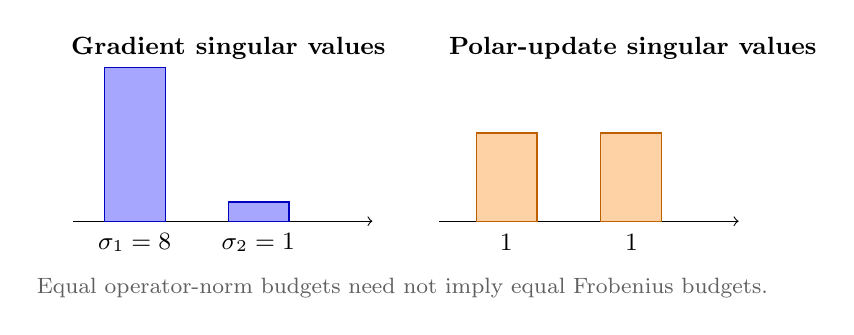
\begin{tikzpicture}[x=1cm,y=1cm,
 bar/.style={fill=blue!35,draw=blue!75!black,line width=.45pt},
 other/.style={fill=orange!35,draw=orange!75!black,line width=.45pt},
 every node/.style={font=\small}]
 \node[anchor=west,font=\bfseries\small] at (.2,2.7) {Gradient singular values};
 \draw[->,thin] (.35,.5)--(4.15,.5);
 \draw[bar] (.75,.5) rectangle (1.52,2.45);
 \draw[bar] (2.32,.5) rectangle (3.09,.744);
 \node at (1.13,.23) {\(\sigma_1=8\)};
 \node at (2.70,.23) {\(\sigma_2=1\)};
 \node[anchor=west,font=\bfseries\small] at (5.0,2.7) {Polar-update singular values};
 \draw[->,thin] (5.0,.5)--(8.8,.5);
 \draw[other] (5.47,.5) rectangle (6.24,1.62);
 \draw[other] (7.05,.5) rectangle (7.82,1.62);
 \node at (5.85,.23) {\(1\)};
 \node at (7.44,.23) {\(1\)};
 \node[font=\footnotesize,gray!75!black] at (4.53,-.35)
   {Equal operator-norm budgets need not imply equal Frobenius budgets.};
\end{tikzpicture}
\caption{The polar factor preserves the singular directions while flattening the nonzero singular values.  Bar heights are schematic; labels give the exact values.}
\label{fig:N20261017-singular-values}
\end{figure}

The example poses a useful question.  Is it better to keep the information in the gradient magnitudes, or to prevent a few large singular modes from swallowing nearly the entire update?  Neither preference makes sense until we decide what constitutes a unit step.

\section{A norm tells us how to spend a step}

For a differentiable loss \(L(W)\), a first-order approximation near \(W\) gives
\[
 L(W+D)=L(W)+\langle G,D\rangle+o(\|D\|),
 \qquad G=\nabla_W L(W).
\]
Fix a radius \(\eta>0\) and a matrix norm \(\|\cdot\|_{\mathcal X}\).  The associated first-order update solves
\begin{equation}
 \min_{\|D\|_{\mathcal X}\leq\eta}\langle G,D\rangle.
 \label{eq:N20261017-linear-oracle}
\end{equation}
Geometrically, we slide a hyperplane perpendicular to \(G\) across a norm ball until it first touches the ball.

In two dimensions, a Euclidean ball is round, while an \(\ell^\infty\) ball is a square.  Their supporting points generally lie in different directions.  The corners of the square make it possible to move at full speed in several coordinates at once.

\begin{figure}[H]
\centering
\begin{tikzpicture}[scale=1.0,>=Latex,every node/.style={font=\small}]
 \begin{scope}[shift={(0,0)}]
  \draw[->] (-1.5,0)--(1.6,0) node[right] {\(d_1\)};
  \draw[->] (0,-1.5)--(0,1.6) node[above] {\(d_2\)};
  \fill[blue!10] (0,0) circle (1.12);
  \draw[blue!70!black,thick] (0,0) circle (1.12);
  \draw[->,very thick,blue!65!black] (0,0)--(-1.02,-.46);
  \node[font=\footnotesize] at (0,-1.82) {Euclidean budget};
 \end{scope}
 \begin{scope}[shift={(4.3,0)}]
  \draw[->] (-1.5,0)--(1.6,0) node[right] {\(d_1\)};
  \draw[->] (0,-1.5)--(0,1.6) node[above] {\(d_2\)};
  \fill[orange!10] (-1.12,-1.12) rectangle (1.12,1.12);
  \draw[orange!80!black,thick] (-1.12,-1.12) rectangle (1.12,1.12);
  \draw[->,very thick,orange!80!black] (0,0)--(-1.12,-1.12);
  \node[font=\footnotesize] at (0,-1.82) {\(\ell^\infty\) budget};
 \end{scope}
 \node[font=\footnotesize,gray!80!black] at (2.15,2.08)
   {Same linear objective, different feasible shapes};
\end{tikzpicture}
\caption{A unit ball is part of the definition of an optimizer's geometry.  The arrows illustrate minimizing directions for a gradient with positive, unequal coordinates; the drawing is schematic.}
\label{fig:N20261017-norm-balls}
\end{figure}

To state the calculation precisely, the \emph{dual norm} is
\[
 \|G\|_{\mathcal X,*}
 =\max_{\|D\|_{\mathcal X}\leq1}\langle G,D\rangle.
\]
Symmetry of a norm ball immediately gives
\begin{equation}
 \min_{\|D\|_{\mathcal X}\leq\eta}\langle G,D\rangle
 =-\eta\|G\|_{\mathcal X,*}.
 \label{eq:N20261017-duality}
\end{equation}
The value comes from the dual norm; a maximizing vector determines the direction.  This distinction matters when a practical optimizer discards the dual-norm magnitude and prescribes a learning rate instead.

For a vector gradient \(g\), the standard cases are easy to check:
\[
 \begin{array}{c|c|c}
 \text{Budget on }d&\text{Optimal direction}&
 \text{First-order reduction per unit radius}\\ \hline
 \|d\|_2\leq1&-g/\|g\|_2&\|g\|_2\\
 \|d\|_\infty\leq1&-\operatorname{sign}(g)&\|g\|_1\\
 \|d\|_1\leq1&-e_j\operatorname{sign}(g_j),\
     j\in\arg\max_i|g_i|&\|g\|_\infty
 \end{array}
\]
Thus the familiar \(\ell^1,\ell^2,\ell^\infty\) geometries make three different decisions: concentrate the budget, preserve the gradient direction, or update all coordinates at full permitted magnitude.  The formula for \(\ell^2\) assumes \(g\ne0\); at \(g=0\) every feasible update minimizes the linear term.

One can also replace the hard constraint by
\[
 \min_D\left\{\langle G,D\rangle+
 \frac{\lambda}{2}\|D\|_{\mathcal X}^2\right\},
 \qquad\lambda>0.
\]
If \(D_1\) is a unit-ball minimizer and \(G\ne0\), the optimum has the form
\begin{equation}
 D_\lambda=\frac{\|G\|_{\mathcal X,*}}{\lambda}D_1.
 \label{eq:N20261017-regularized-descent}
\end{equation}
Indeed, any \(D=rT\) with \(\|T\|_{\mathcal X}=1\) reduces the problem to minimizing
\(-r\|G\|_{\mathcal X,*}+\lambda r^2/2\).
Choosing a \emph{direction} by a norm and choosing its \emph{scale} by a learning-rate schedule are separable modeling decisions.\footnote{The geometric viewpoint follows Jeremy Bernstein and Laker Newhouse, \href{https://arxiv.org/abs/2409.20325}{\emph{Old Optimizer, New Norm: An Anthology}} (2024).  The steepest-descent identities used here also follow directly from finite-dimensional norm duality.}

\section{Which two-norm? A matrix has several}

We should settle a terminological trap before going further.  For a vector, \(\|x\|_2\) has an unambiguous meaning.  For a matrix \(A\in\mathbb R^{m\times n}\), both of these are common:
\[
 \|A\|_{\mathrm F}
 =\left(\sum_{i,j}A_{ij}^2\right)^{1/2},
 \qquad
 \|A\|_{\mathrm{op}}
 =\max_{x\ne0}\frac{\|Ax\|_2}{\|x\|_2}.
\]
The first treats a matrix as a long vector of \(mn\) entries.  The second treats it as an operator on input activations.  Some authors write \(\|A\|_2\) for the \emph{second} quantity, even though the first is the Schatten-\(2\) norm.

If \(A=U\operatorname{diag}(\sigma_1,\ldots,\sigma_r)V^\top\) is a compact singular value decomposition, then
\[
 \|A\|_{\mathrm{op}}=\max_i\sigma_i,\qquad
 \|A\|_{\mathrm F}=\Bigl(\sum_i\sigma_i^2\Bigr)^{1/2},
 \qquad
 \|A\|_*=\sum_i\sigma_i.
\]
Here \(\|\cdot\|_*\) is the nuclear or trace norm.  For the matrix of all ones in dimension \(n\),
\[
 \|A\|_{\mathrm{op}}=n,\qquad
 \|A\|_{\mathrm F}=n,\qquad
 \|A\|_*=n;
\]
but for the identity \(I_n\),
\[
 \|I_n\|_{\mathrm{op}}=1,\qquad
 \|I_n\|_{\mathrm F}=\sqrt n,\qquad
 \|I_n\|_*=n.
\]
The identity has no particularly large effect on any \emph{single} input direction.  Nevertheless, it acts nontrivially on \emph{all} \(n\) directions, a distinction detected by the Frobenius and nuclear norms.

These quantities are special cases of the Schatten norms
\[
 \|A\|_{S_p}=\left(\sum_i\sigma_i^p\right)^{1/p},
 \quad 1\leq p<\infty,
 \qquad
 \|A\|_{S_\infty}=\max_i\sigma_i.
\]
In particular, \(S_2\) is the Frobenius norm and \(S_\infty\) is the spectral norm.  The phrase about learning in a Euclidean two-norm rather than a spectral norm only becomes meaningful once this distinction is fixed.

\section{Why spectral steepest descent is a matrix sign}

The dual norm of the spectral norm is the nuclear norm.  An especially transparent proof also gives the update direction.

\begin{proposition}
Let \(G\in\mathbb R^{m\times n}\) have compact SVD
\(
 G=U_r\operatorname{diag}(\sigma_1,\ldots,\sigma_r)V_r^\top
\),
where \(\sigma_i>0\).  Then
\[
 \min_{\|D\|_{\mathrm{op}}\leq\eta}
       \langle G,D\rangle
 =-\eta\sum_{i=1}^r\sigma_i,
\]
and a minimizer is
\begin{equation}
 D_{\mathrm{sp}}=-\eta U_rV_r^\top.
 \label{eq:N20261017-matrix-sign}
\end{equation}
\end{proposition}

\begin{proof}
Write \(u_i,v_i\) for the singular vectors.  For every admissible \(D\),
\[
 \langle G,D\rangle
 =\sum_i\sigma_i\,u_i^\top Dv_i
 \geq-\sum_i\sigma_i\|Dv_i\|_2
 \geq-\eta\sum_i\sigma_i.
\]
For \(D=-\eta U_rV_r^\top\), the identity \(U_r^\top U_r=V_r^\top V_r=I_r\)
shows \(Dv_i=-\eta u_i\), so both inequalities are equalities.
\end{proof}

The matrix \(U_rV_r^\top\) is the \emph{partial polar factor}, also called the matrix sign in this context.  All its nonzero singular values are \(1\).  For an invertible square matrix, it is orthogonal; for a rectangular matrix, it has orthonormal columns or rows on the relevant subspace.  There is no requirement that the weight matrix itself become orthogonal.

Contrast this with the Frobenius-constrained solution:
\[
 D_{\mathrm F}=-\eta\frac{G}{\|G\|_{\mathrm F}}.
\]
The spectral optimizer keeps the singular vectors and flattens the singular values; the Frobenius optimizer keeps the ratios between singular values.  Both are exact optimizers of their respective \emph{linearized} problems.

We also have a precise answer to the opening calculation.  For
\(G=\operatorname{diag}(8,1)\), spectral descent gives \(-\eta I_2\), while
Frobenius descent gives \(-\eta\operatorname{diag}(8,1)/\sqrt{65}\).  The gradient-scaled step of our opening example used a \emph{spectral}, rather than Frobenius, radius.  Comparing the three objects prevents two meanings of a normalized gradient from being conflated.

\section{Between preserving and erasing the spectrum}

The difference between those two updates suggests that the choice need not be all-or-nothing.  For \(1<p<\infty\), write \(q=p/(p-1)\).  Schatten-\(p\) and Schatten-\(q\) norms are dual, just as vector \(\ell^p\) and \(\ell^q\) norms are dual.

\begin{proposition}
Under the constraint \(\|D\|_{S_p}\leq\eta\), one optimal update is
\begin{equation}
 D_p=-\eta U_r
 \operatorname{diag}\left(
 \frac{\sigma_i^{q-1}}{(\sum_j\sigma_j^q)^{1/p}}
 \right)_{i=1}^rV_r^\top.
 \label{eq:N20261017-schatten-step}
\end{equation}
Its first-order decrease is \(-\eta\|G\|_{S_q}\).
\end{proposition}

\begin{proof}
The singular-value inequality gives
\(\langle G,D\rangle\geq-\sum_i\sigma_i s_i(D)\).
By H\"older's inequality,
\[
 \sum_i\sigma_i s_i(D)
 \leq\left(\sum_i\sigma_i^q\right)^{1/q}
      \left(\sum_i s_i(D)^p\right)^{1/p}.
\]
Equality holds when the singular vectors are aligned in opposite
directions and \(s_i(D)\) is proportional to \(\sigma_i^{q-1}\).
Setting the \(p\)-norm of that singular-value vector to \(\eta\)
gives the stated normalization.
\end{proof}

It is illuminating to suppress the overall scalar and look only at
\[
 \Psi_a(G)=U_r\operatorname{diag}(\sigma_i^a)V_r^\top,
 \qquad 0\leq a\leq1.
\]
When \(a=1\), the spectral magnitudes are preserved.  When \(a=0\), every nonzero singular value becomes \(1\).  Intermediate exponents gently compress the dynamic range.  More precisely, the \emph{direction} \(\Psi_a(G)\) is that of Schatten-\(p\) steepest descent for \(p=1+1/a\), when \(a>0\); the limit \(a\to0\) corresponds to \(S_\infty\).

For our two-singular-value example:
\[
 \begin{array}{c|c|c}
 a&\text{relative singular magnitudes}&
         \text{ratio of large to small}\\ \hline
 1&(8,1)&8\\
 1/2&(\sqrt8,1)&\sqrt8\\
 1/4&(8^{1/4},1)&8^{1/4}\\
 0&(1,1)&1
 \end{array}
\]
This is a family of \emph{directions}.  A practical implementation must still say how the direction is normalized and how the step size is selected.

There is an important caveat.  Applying \(\Psi_a\) to a momentum estimate, or to an Adam-normalized update, is not generally the same as solving the original loss's steepest-descent problem in a single fixed Schatten geometry.  The transformed input already depends on optimization history.  The spectral family remains useful precisely because it lets us study \emph{how much} of that input's spectrum should be kept.

\section{AdamW lives in moving coordinates}

Let \(g_t\) be the stochastic gradient at iteration \(t\); write all products and divisions below entrywise.  Adam maintains
\[
 \begin{aligned}
 m_t&=\beta_1m_{t-1}+(1-\beta_1)g_t,\\
 v_t&=\beta_2v_{t-1}+(1-\beta_2)g_t\odot g_t,\\
 \widehat m_t&=\frac{m_t}{1-\beta_1^t},
 \qquad
 \widehat v_t=\frac{v_t}{1-\beta_2^t}.
 \end{aligned}
\]
With decoupled weight decay, the update is
\begin{equation}
 W_{t+1}=(1-\eta_t\lambda)W_t
 -\eta_t\frac{\widehat m_t}{\sqrt{\widehat v_t}+\varepsilon}.
 \label{eq:N20261017-adamw}
\end{equation}
The first state tracks a preferred direction; the second tracks the recent size of gradient coordinates.  Coordinates with large historical squared gradients are damped.

It would be inaccurate to say that full AdamW is simply Euclidean gradient descent.  Freeze \(v_t\), set \(D_t=\operatorname{diag}((\sqrt{\widehat v_{t,i}}+\varepsilon)^{-1})\) after vectorizing the matrix, and ignore weight decay.  The update is then
\[
 d_t=-\eta_tD_t\widehat m_t.
\]
This is the minimizer of
\begin{equation}
 \min_d\left\{\widehat m_t^\top d+
         \frac{1}{2\eta_t}d^\top D_t^{-1}d\right\}.
 \label{eq:N20261017-adam-metric}
\end{equation}
Thus, at a frozen instant, Adam behaves like steepest descent in a \emph{weighted quadratic geometry}.  The geometry moves with \(v_t\); the momentum \(\widehat m_t\) is also generally different from the instantaneous gradient.  Equation \eqref{eq:N20261017-adam-metric} is an interpretation of the direction conditional on these states, not an exact static-norm description of the entire Adam trajectory.

There is a second, simpler connection.  If \(\beta_1=\beta_2=0\) and \(\varepsilon=0\) on nonzero gradient coordinates, Adam's update direction is
\[
 \frac{g_t}{\sqrt{g_t\odot g_t}}
 =\operatorname{sign}(g_t).
\]
This is the \(\ell^\infty\)-budget direction from our norm-ball picture.  With realistic momentum and second-moment estimates, however, Adam's direction need not be a sign vector.

The distinction is both mathematically and experimentally important.  Muon and AdamW do not form a clean opposition between spectral norm and ordinary \(L^2\).  A cleaner comparison is between \emph{spectral normalization of a matrix-valued momentum} and \emph{history-dependent coordinatewise preconditioning}.  Their norm geometries are related but their actual optimization procedures contain additional ingredients.

\section{Muon orthogonalizes a momentum matrix}

For a hidden matrix \(W_t\), a typical Muon step maintains one momentum buffer
\[
 M_t=\beta M_{t-1}+G_t
\]
and forms a Nesterov-style combination such as
\(\widetilde M_t=\beta M_t+G_t\).
It then computes an approximation to the polar factor
\[
 \operatorname{polar}(\widetilde M_t)
 =U_rV_r^\top
\]
and uses a shape-dependent scale \(s_{m,n}\):
\begin{equation}
 W_{t+1}=(1-\eta_t\lambda)W_t
 -\eta_t s_{m,n}\,\operatorname{polar}(\widetilde M_t).
 \label{eq:N20261017-muon}
\end{equation}
Momentum conventions, the exact normalization of the gradient, weight decay and scaling factors vary across implementations.  It is the \emph{polar operation on a matrix update} that identifies the family.

Why not compute a full SVD at every step?  Muon uses a small number of Newton--Schulz-type matrix iterations.  Starting with a normalized matrix \(X_0\), a popular form applies a polynomial
\begin{equation}
 X_{k+1}=aX_k+b(X_kX_k^\top)X_k+
               c(X_kX_k^\top)^2X_k.
 \label{eq:N20261017-NS}
\end{equation}
If \(X_k=U\operatorname{diag}(s_i)V^\top\), the next iterate has the same singular vectors and transformed singular values
\[
 s_i\longmapsto a s_i+b s_i^3+c s_i^5.
\]
We can think of the iteration as repeatedly redrawing the \emph{heights} of the singular-value bars, ideally pushing them toward a common level.  The real computation uses matrix multiplications and avoids explicitly extracting those bars.

A finite number of polynomial iterations only \emph{approximates} the polar factor.  The approximation can also matter for small singular values; the different published coefficient choices and scaling rules should not be treated as mathematically identical.  In particular, the efficient GPU implementation is an algorithmic achievement in its own right, distinct from the abstract solution of a spectral-norm trust-region problem.

The standard practice is hybrid: Muon handles selected two-dimensional hidden weights, while embeddings, normalization scales, biases and frequently the output head remain on AdamW.  A Transformer therefore uses more than one update geometry at the same time.

The polar step also does not make second-moment information intrinsically useless.  For example, the 2026 preprint \href{https://arxiv.org/abs/2604.09967}{\emph{Muon\textsuperscript{2}}} applies an Adam-style second-moment preconditioner \emph{before} orthogonalization, partly to improve the conditioning of Newton--Schulz inputs.  Its factorized variant trades additional state against cheaper approximations.  This is a different algorithm from the one-state Muon discussed here, and is another reason to separate geometry from implementation.

\section{The memory advantage has an exact accounting}

Suppose a hidden weight matrix contains \(N=mn\) parameters and its optimizer states are stored in 32-bit floating-point numbers.  Ignoring distributed sharding, the persistent state count for that matrix is
\[
 \begin{array}{c|c|c}
 \text{Optimizer on the matrix}&\text{Persistent state tensors}&
      \text{State bytes}\\ \hline
 \text{AdamW}&m_t,\;v_t&8N\\
 \text{Muon}&M_t&4N
 \end{array}
\]
That is a genuine reduction of \emph{one full state tensor} for eligible matrix parameters.  It does not require any claim about validation loss to be valuable.

For a concrete scale, a matrix with \(N=10^8\) entries costs about \(800\) MB of such AdamW optimizer state and \(400\) MB of Muon momentum state (decimal megabytes).  But this is deliberately a \emph{state-only} calculation.

Real training also stores parameter values, gradients, possibly FP32 master weights, activations, communication buffers and allocator overhead.  Muon's matrix iterations require temporary workspace, and the nonmatrix parameters still use AdamW.  ZeRO or tensor parallelism can change which rank holds the persistent state and how frequently it is communicated.  Therefore the per-matrix state saving is certain under the stated storage assumptions; a particular reduction in \emph{peak GPU memory} must be measured rather than inferred by multiplying the number of model parameters by four bytes.

A similar separation is needed for speed.  Muon can use fewer optimization steps to reach a loss threshold and still take more time per step, because its orthogonalization involves extra matrix multiplications.  The two comparisons to report are
\[
 \text{loss versus tokens seen},
 \qquad
 \text{loss versus actual wall-clock time}.
\]
The first measures sample efficiency; the second captures the computer on which one actually trains.

\section{Why rectangular matrices need different scales}

Even a perfect polar factor has a surprisingly shape-dependent \emph{entrywise} size.  Let \(P=U_rV_r^\top\) be the polar factor of a rank-\(r\) matrix of shape \(m\times n\).  Since the singular values of \(P\) are \(1\) on its active rank,
\[
 \|P\|_{\mathrm F}^2=r.
\]
Define the root-mean-square entry magnitude by
\(
 \operatorname{RMS}(P)=\|P\|_{\mathrm F}/\sqrt{mn}.
\)
We obtain the exact identity
\begin{equation}
 \operatorname{RMS}(P)=\sqrt{\frac{r}{mn}}.
 \label{eq:N20261017-polar-rms}
\end{equation}
For a full-rank matrix, \(r=\min(m,n)\), so
\begin{equation}
 \operatorname{RMS}(P)=\frac{1}{\sqrt{\max(m,n)}}.
 \label{eq:N20261017-full-rank-rms}
\end{equation}

A square \(d\times d\) hidden matrix has polar-update RMS \(1/\sqrt d\).  A \(d\times4d\) expansion matrix has RMS \(1/(2\sqrt d)\).  If we used the same raw multiplier for both, the rectangular layer would receive an update with half the RMS, even though the matrices are participating in the same network.

Multiplying by \(\sqrt{\max(m,n)}\) aligns the full-rank RMS at \(1\).  Liu and collaborators use a multiplier of the form \(0.2\sqrt{\max(m,n)}\) to aim for an AdamW-like update RMS in their training recipe.  The factor \(0.2\) is an \emph{empirical scale choice}; the square-root dimension factor follows from the rank calculation.

Two cautions follow.  The formula is exact for the ideal rank-\(r\) polar factor, while practical Newton--Schulz outputs have approximately flattened singular values.  And equal RMS does not mean equal effect on the network.  The latter issue takes us from the optimizer to the actual role of a matrix.

\section{A layer is a map, not a table of parameters}

A hidden linear layer transforms an activation \(x\in\mathbb R^{d_{\mathrm{in}}}\) into
\[
 y=Wx,\qquad W\in\mathbb R^{d_{\mathrm{out}}\times d_{\mathrm{in}}}.
\]
If the parameters change by \(D\), the layer output changes by
\[
 \delta y=Dx.
\]
The spectral norm has a direct functional meaning:
\begin{equation}
 \sup_{x\ne0}\frac{\|Dx\|_2}{\|x\|_2}=\|D\|_{\mathrm{op}}.
 \label{eq:N20261017-operator-gain}
\end{equation}
Constraining \(\|D\|_{\mathrm{op}}\) limits the worst amplification of an input through the update map.  It is a plausible geometric prior for a linear layer whose inputs and outputs are measured by Euclidean norms.

This argument is suggestive, not conclusive.  Embedding tables are typically used by \emph{selecting rows}, not by multiplying arbitrary dense input vectors.  Attention weights are embedded in bilinear interactions, a softmax, and residual connections.  Normalization parameters act by coordinatewise multiplication.  Treating every parameter block as an arbitrary linear operator throws away those different roles.

Even among linear maps, the notion of a unit step can depend on width.  A vector RMS is
\[
 \|x\|_{\mathrm{rms}}=\frac{\|x\|_2}{\sqrt{d_{\mathrm{in}}}},
 \qquad
 \|y\|_{\mathrm{rms}}=\frac{\|y\|_2}{\sqrt{d_{\mathrm{out}}}}.
\]
The induced RMS-to-RMS operator norm is
\begin{equation}
 \|D\|_{\mathrm{rms}\to\mathrm{rms}}
 =\sqrt{\frac{d_{\mathrm{in}}}{d_{\mathrm{out}}}}\,
       \|D\|_{\mathrm{op}}.
 \label{eq:N20261017-rms-operator}
\end{equation}
Thus a stable worst-case \emph{RMS} effect across rectangular layers suggests a width correction.  The appropriate factor depends on which spaces and normalization conventions we regard as physically meaningful.  This is one reason that matrix shapes and parameterization rules must be part of a serious optimizer comparison.

\section{The same network can have very different coordinates}

There is a simple obstruction to choosing an optimizer geometry from flattened parameters alone.  Consider a two-layer linear network,
\[
 f(x)=W_2W_1x.
\]
For any nonzero scalar \(c\),
\[
 W_1'=cW_1,\qquad W_2'=c^{-1}W_2
\]
produces exactly the same function.  Yet an entrywise or Frobenius update with the same raw numerical scale can have a different effect in these new coordinates.

To see this without matrix notation, set \(f(x)=abx\) with scalar parameters \(a,b\).  Let the loss depend on \(z=ab\) through some differentiable function \(\ell(z)\).  Its parameter gradients are
\[
 \frac{\partial L}{\partial a}=b\ell'(ab),
 \qquad
 \frac{\partial L}{\partial b}=a\ell'(ab).
\]
Under the equivalent parameterization \(a'=ca,\ b'=b/c\), these become
\[
 \frac{\partial L}{\partial a'}=\frac{b}{c}\ell'(ab),
 \qquad
 \frac{\partial L}{\partial b'}=ca\ell'(ab).
\]
Euclidean gradient descent therefore takes different \emph{functional} steps in two descriptions of the same current model.  Indeed, to first order,
\[
 \delta z=b\,\delta a+a\,\delta b,
\]
and the two gradient steps induce
\[
 \delta z=-\eta(a^2+b^2)\ell'(z),\qquad
 \delta z'=-\eta\left(c^2a^2+\frac{b^2}{c^2}\right)\ell'(z).
\]
For large \(c\), the second expression may be arbitrarily larger.  The ambiguity is already present in the simplest possible neural network.

This calculation does not prove that there exists one perfectly parameterization-invariant practical optimizer for modern Transformers.  It does show why geometry tied to the \emph{function performed} by the model is a more principled target than geometry assigned solely to a list of entries.

\section{Typical activations and worst-case activations disagree}

The spectral norm considers the worst input direction.  But the training data do not necessarily explore every direction equally often.

Let \(x\) have finite second moment \(C_x=\mathbb E[xx^\top]\), which is positive semidefinite.  The expected squared output change caused by \(D\) is
\begin{align}
 \mathbb E\|Dx\|_2^2
 &=\mathbb E[x^\top D^\top Dx]\notag\\
 &=\operatorname{tr}\bigl(D^\top D\,\mathbb E[xx^\top]\bigr)\notag\\
 &=\operatorname{tr}(DC_xD^\top)
 =\|DC_x^{1/2}\|_{\mathrm F}^2.
 \label{eq:N20261017-covariance-metric}
\end{align}
This is an exact identity, with no Gaussian assumption.  If the mean of \(x\) is nonzero, \(C_x\) is the \emph{second-moment} matrix; it is not the centered covariance unless the mean is zero.

For a numerical example, suppose
\[
 C_x=\begin{pmatrix}100&0\\0&1\end{pmatrix},\qquad
 D_1=\varepsilon\begin{pmatrix}1&0\\0&0\end{pmatrix},
 \qquad
 D_2=\varepsilon\begin{pmatrix}0&0\\0&1\end{pmatrix}.
\]
Both updates have operator norm \(|\varepsilon|\) and Frobenius norm \(|\varepsilon|\).  Yet
\[
 \mathbb E\|D_1x\|_2^2=100\varepsilon^2,\qquad
 \mathbb E\|D_2x\|_2^2=\varepsilon^2.
\]
A unit update in a frequently excited input direction can be a hundred times as consequential, in expected squared output change, as the same-sized update in a quiet direction.

\begin{figure}[H]
\centering
\begin{tikzpicture}[>=Latex,every node/.style={font=\small}]
 \node[draw,rounded corners=1.5pt,minimum height=1cm,minimum width=2.5cm,
  fill=blue!6,align=center] (x) at (0,0)
  {Inputs \(x\)\\\(\mathbb E[xx^\top]=C_x\)};
 \node[draw,rounded corners=1.5pt,minimum height=1cm,minimum width=2cm,
  fill=orange!8,align=center] (d) at (4.1,0)
  {Update \(D\)\\\(x\mapsto Dx\)};
 \node[draw,rounded corners=1.5pt,minimum height=1cm,minimum width=3.0cm,
  fill=green!7,align=center] (y) at (8.45,0)
  {Output disturbance\\\(\mathbb E\|Dx\|_2^2\)};
 \draw[->,thick] (x)--(d);
 \draw[->,thick] (d)--(y);
 \node[font=\footnotesize,gray!75!black,align=center] at (4.2,-1.0)
  {\(\operatorname{tr}(DC_xD^\top)\) weighs an update\\by the directions the inputs actually visit.};
\end{tikzpicture}
\caption{An input-dependent geometry counts how the update acts on the observed activation distribution.  Operator norm instead bounds the most amplified direction, whether or not that direction is common.}
\label{fig:N20261017-input-geometry}
\end{figure}

If \(C_x=I\), the data-weighted norm reduces to Frobenius norm.  If \(C_x\) is strongly anisotropic, an unweighted Frobenius ball can be a poor model of functional change.  The spectral norm remains valuable as a worst-case bound, but the example explains why it should not automatically be called the unique natural geometry of training.

\section{From change in activations to change in loss}

Even equal output disturbance need not mean equal \emph{loss} disturbance.  Some output directions are much more consequential than others.

Let a layer's output be \(y=Wx\), and suppose that, for a particular input \(x\), a smooth local loss as a function of \(y\) has Hessian \(H_y(x)\).  Its second-order response to \(D\) contains the term
\begin{equation}
 \frac12\mathbb E_x\left[
 (Dx)^\top H_y(x)(Dx)\right].
 \label{eq:N20261017-functional-curvature}
\end{equation}
An arbitrary Hessian need not be positive semidefinite; a positive metric is obtained only when one uses an appropriate positive-semidefinite curvature surrogate, such as a Gauss--Newton or Fisher-type matrix.

In the instructive case where a fixed positive-definite output metric \(A\) is appropriate and the input second moment is \(B=C_x\), the associated quadratic size becomes
\begin{equation}
 \|D\|_{A,B}^2
 =\operatorname{tr}(ADBD^\top)
 =\|A^{1/2}DB^{1/2}\|_{\mathrm F}^2.
 \label{eq:N20261017-two-sided-metric}
\end{equation}
The input side accounts for \emph{where the network is used}; the output side accounts for \emph{which changes matter}.  This is a concrete reason to consider geometry on \emph{both} sides of a weight matrix.

There is a familiar connection to natural gradient.  A Fisher quadratic form measures the local change in a model's predictive distribution, often expressed through a second-order approximation to a Kullback--Leibler divergence.  Kronecker-factored approximations in layered networks replace a large curvature matrix by smaller input and output factors.  The product form \eqref{eq:N20261017-two-sided-metric} has the same algebraic shape.

But the factorization is an \emph{approximation} in general: the exact expectation of \(H_y(x)\otimes xx^\top\) need not equal the product of the expectations.  A metric estimated from minibatches may also be singular or noisy.  None of these equations declares an optimizer optimal before its estimation cost and errors have been accounted for.

\section{The layers also compete for an update budget}

Even after selecting a norm for each matrix, we must decide how to combine them.  A network parameter space is a product:
\[
 \Theta=\mathbb R^{m_1\times n_1}\times\cdots\times
         \mathbb R^{m_L\times n_L}\times
         \text{(vector and scalar parameters)}.
\]
For simplicity, take just the matrix factors, with gradient \(G_\ell\) at layer \(\ell\), and consider the weighted product norm
\[
 \|D\|_{\mathrm{block}}^2
 =\sum_{\ell=1}^L a_\ell\|D_\ell\|_{\mathrm{op}}^2,
 \qquad a_\ell>0.
\]
The regularized first-order model is separable:
\begin{equation}
 \min_{D_1,\ldots,D_L}
 \sum_{\ell=1}^L\langle G_\ell,D_\ell\rangle+
 \frac{\lambda}{2}\sum_{\ell=1}^L
 a_\ell\|D_\ell\|_{\mathrm{op}}^2.
 \label{eq:N20261017-layer-aggregation}
\end{equation}

Using the single-matrix duality result, a minimizer for every nonzero \(G_\ell\) is
\begin{equation}
 D_\ell=-\frac{\|G_\ell\|_*}{\lambda a_\ell}\,
                \operatorname{polar}(G_\ell).
 \label{eq:N20261017-block-solution}
\end{equation}
In other words, a matrix's polar factor fixes its \emph{direction}, while the weight \(a_\ell\) and the layerwise nuclear norm decide \emph{how much of the network budget} that matrix receives.

Compare this with a separate rule assigning each layer exactly the same scalar learning rate.  Such a rule can use the same polar \emph{directions}, yet it generally does not solve \eqref{eq:N20261017-layer-aggregation}.  With two layers whose gradient nuclear norms are \(10\) and \(1\), respectively, the first-order model with equal \(a_\ell\) allots ten times the spectral step magnitude to the first layer.  Equal fixed per-layer radii allot them equal magnitudes instead.

There is no theorem saying that proportional-to-gradient budgets will train an LLM best; it is an exact result for a particular local model.  It exposes a choice that is easy to mistake for a mere implementation detail: \emph{how are the norms of different modules aggregated?}

Recent studies make this issue concrete.  Crawshaw and collaborators explore product norms and Muon variants with improved learning-rate robustness; He and collaborators demonstrate that learning rates adapted to layers' spectral statistics can help \emph{both} Muon and AdamW.  Better layerwise step allocation is therefore a serious alternative explanation for some improvements attributed entirely to the matrix orthogonalization operation.\footnote{See Michael Crawshaw and collaborators, \href{https://proceedings.mlr.press/v306/crawshaw26a.html}{\emph{An Exploration of Non-Euclidean Gradient Descent: Muon and its Many Variants}} (ICML 2026), and Di He and collaborators, \href{https://proceedings.mlr.press/v306/he26ak.html}{\emph{One LR Doesn't Fit All}} (ICML 2026).}

\section{A small singular value can carry loud noise}

There is a second, less obvious difficulty with full spectral flattening: polar normalization may treat a tiny component as though it were as reliable as a large one.

Consider
\[
 G_\delta=\begin{pmatrix}1&0\\0&\delta\end{pmatrix},
 \qquad \delta\ne0.
\]
Its partial polar factor is
\[
 \operatorname{polar}(G_\delta)
 =\begin{pmatrix}1&0\\0&\operatorname{sign}(\delta)\end{pmatrix}.
\]
Changing \(\delta\) from \(10^{-6}\) to \(-10^{-6}\) changes the gradient matrix by only \(2\cdot10^{-6}\) in Frobenius norm.  Yet it changes the polar factor by \(2\) in operator norm.  As \(\delta\to0^\pm\), the two one-sided polar limits disagree.

This is an exact discontinuity in the ideal matrix sign at a rank change.  It does \emph{not} prove that a particular finite-step Muon implementation is unstable: the polynomial iteration, momentum, gradient noise distribution and finite precision all influence what happens.  It does reveal an obvious potential cost of discarding the magnitude of every small singular component.  A weak, unreliable singular mode may be raised to a full-sized update direction.

Partially compressing the spectrum, clipping a few large spectral spikes, or applying coordinatewise RMS normalization before spectral processing are different responses to this issue.  They answer distinct questions: should we suppress dominant modes, preserve small ones, or estimate their reliability first?

\section{Why a larger first-order win can lose the actual step}

A more dramatic example shows why the best \emph{linearized} update need not be the best finite update.  Consider an exact quadratic loss in two parameters,
\[
 \ell(z_1,z_2)
 =8z_1+z_2+\frac12\bigl(z_1^2+100z_2^2\bigr),
 \qquad z=(0,0).
\]
The gradient at the origin is \(g=(8,1)\).  Put these parameters on the diagonal of a \(2\times2\) matrix; the two singular directions are then precisely the coordinate axes.  The curvature of the second direction is a hundred times that of the first.

At an operator-norm step budget of \(\eta=0.1\), consider
\[
 D_{\mathrm{polar}}=-0.1\operatorname{diag}(1,1),
 \qquad
 D_{\mathrm{scaled}}=-0.1\operatorname{diag}(1,1/8).
\]
Both have operator norm \(0.1\).  The polar step wins on the first-order term:
\[
 \langle G,D_{\mathrm{polar}}\rangle=-0.9,\qquad
 \langle G,D_{\mathrm{scaled}}\rangle=-0.8125.
\]

\begin{figure}[H]
\centering
\begin{tikzpicture}[x=24cm,y=24cm,>=Latex,every node/.style={font=\small}]
 \draw[->] (-.155,0)--(.075,0) node[right] {\(z_1\)};
 \draw[->] (0,-.135)--(0,.11) node[above] {\(z_2\)};
 \foreach \r in {.35,.65,1}{
   \draw[gray!50] (0,0) ellipse ({.105*\r} and {.0105*\r});
 }
 \fill (0,0) circle (.65pt) node[above right] {\(0\)};
 \draw[->,very thick,orange!85!black] (0,0)--(-.10,-.10);
 \draw[->,very thick,blue!75!black] (0,0)--(-.10,-.0125);
 \fill[orange!85!black] (-.1,-.1) circle (.72pt);
 \fill[blue!75!black] (-.1,-.0125) circle (.72pt);
 \node[font=\footnotesize,orange!75!black,anchor=north] at (-.103,-.101)
   {polar};
 \node[font=\footnotesize,blue!70!black,anchor=south] at (-.103,-.008)
   {scaled gradient};
 \node[font=\footnotesize,gray!75!black,anchor=west,align=left] at (.085,.07)
   {Curvature is\\much sharper\\vertically.};
\end{tikzpicture}
\caption{Two updates of equal spectral norm on the explicitly specified quadratic.  Ellipses indicate the \emph{curvature part} \(\frac12(z_1^2+100z_2^2)\), centered at the origin; the full loss has additional linear terms.}
\label{fig:N20261017-curvature-counterexample}
\end{figure}
But the \emph{actual} loss changes are
\begin{align*}
 \ell(-0.1,-0.1)-\ell(0,0)
 &= -0.9+\frac12(0.01+100\cdot0.01)
 =-0.395,\\
 \ell(-0.1,-0.0125)-\ell(0,0)
 &= -0.8125+\frac12(0.01+100\cdot0.0125^2)
 =-0.7996875.
\end{align*}
The step with the \emph{worse first-order prediction} lowers the true quadratic loss by roughly twice as much.  Every number here comes from the stated quadratic; there is no neural-network experiment hidden inside the example.

What happened?  The polar step spent much of its second-order curvature budget moving in the \(z_2\) direction, where even a small displacement is expensive.  In general,
\begin{equation}
 L(W+D)-L(W)
 \approx \langle G,D\rangle+
 \frac12\,\operatorname{vec}(D)^\top
 H_W\,\operatorname{vec}(D).
 \label{eq:N20261017-curvature-balance}
\end{equation}
One can factor the second-order term as
\[
 \frac12\|D\|_{\mathrm F}^2
 \underbrace{\frac{\operatorname{vec}(D)^\top
 H_W\operatorname{vec}(D)}{\|D\|_{\mathrm F}^2}}_
 {\text{directional curvature, for }D\ne0}.
\]
Thus a method can make a favorable first-order step, yet incur a large curvature penalty.  The Hessian need not be positive in general; here it is positive definite, so the mechanism is particularly clear.



Shuche Wang and collaborators report smaller normalized directional sharpness for Muon than for Adam in their studied language-model settings.\footnote{See \href{https://arxiv.org/abs/2606.04662}{\emph{Why Muon Outperforms Adam: A Curvature Perspective}} (2026 preprint).}  That finding makes a plausible bridge from spectral update geometry to faster training, but it is an empirical and model-dependent observation.  The quadratic above explains why such a curvature comparison is worth making, and why one should not infer a universally superior optimizer solely from the matrix sign formula.

\section{Early speed, eventual loss, and model quality}

Several different empirical statements tend to be rolled together when discussing new optimizers.  We should pull them apart.

\emph{First}, reaching a validation-loss threshold in fewer tokens is a claim about data or optimization-step efficiency.  \emph{Second}, reaching it in less wall-clock time also depends on kernel speed, precision, communication and sharding.  \emph{Third}, reaching a smaller final loss depends on the training horizon, learning-rate schedule, weight decay, regularization and tuning budget.  \emph{Fourth}, a model's useful capabilities may not be accurately ordered by a small difference in aggregate next-token loss.

The published record illustrates these distinctions:

\begin{itemize}
 \item In the large-scale Moonlight study, Muon was made practical with weight decay and matrix-shape-aware scaling, and showed strong training-efficiency results.  Those findings concern a particular distributed implementation and training recipe.
 \item Wen, Hall, Ma and Liang compared optimizers across several language-model scales and training horizons with more systematic hyperparameter searches.  They found that rankings can change between intermediate and final checkpoints; the advantage over tuned AdamW narrows at larger model sizes in their evaluated regime.
 \item Qi and collaborators evaluated a family \(U\Sigma^aV^\top\) on a controlled \(124\)M-parameter GPT-2 setup.  In that setting, the completely flattened momentum update was not consistently best.  RMS-normalized inputs and partial spectral compression were competitive, and the amount of compression mattered.
 \item Layerwise learning-rate studies and product-norm studies show that a large part of the optimization problem lies \emph{outside} the normalization of any one matrix: how the method distributes step sizes over heterogeneous layers changes the comparison.
\end{itemize}

These observations are compatible.  A method may win on the time needed to reach an early loss threshold, show a narrow final loss advantage under a different budget, and yield models whose downstream accuracies are statistically indistinguishable on the tested tasks.  A good comparison must say which outcome matters and hold the other resources approximately fixed.

In particular, tuning one AdamW learning rate globally and giving Muon separate matrix/vector learning rates is an unfair test of the full recipes.  But assigning separate learning rates to \emph{every} AdamW layer also costs tuning resources, and Muon may benefit from the same freedom.  A credible comparison reports its search space, search cost and held-out selection rule.\footnote{For controlled optimizer comparisons, see Kaiyue Wen, David Hall, Tengyu Ma and Percy Liang, \href{https://arxiv.org/abs/2509.02046}{\emph{Fantastic Pretraining Optimizers and Where to Find Them}} (ICLR 2026), and Xianbiao Qi and collaborators, \href{https://proceedings.mlr.press/v306/qi26c.html}{\emph{Delving into Muon and Beyond}} (ICML 2026).  Their setups and conclusions should not be collapsed into a single universal speedup.}

\section{A more meaningful matrix geometry}

We can now make a constructive guess.  If the input statistics \(B\) and output sensitivity \(A\) matter, perhaps a useful update norm should be placed on
\[
 Z=A^{1/2}DB^{1/2}
\]
rather than on the raw entries of \(D\).

This suggestion leads to two precise first-order models.  Suppose for the moment that \(A\in\mathbb R^{m\times m}\) and \(B\in\mathbb R^{n\times n}\) are symmetric positive definite and held fixed during the step.

\emph{A data-weighted quadratic budget.}  Consider
\begin{equation}
 \min_D\left\{\langle G,D\rangle+
      \frac{\lambda}{2}\|A^{1/2}DB^{1/2}\|_{\mathrm F}^2\right\}.
 \label{eq:N20261017-weighted-quadratic}
\end{equation}
Differentiating with respect to \(D\) gives
\[
 G+\lambda ADB=0.
\]
Hence
\begin{equation}
 D_{\mathrm{quad}}=-\frac{1}{\lambda}A^{-1}GB^{-1}.
 \label{eq:N20261017-two-sided-preconditioner}
\end{equation}
This is a two-sided preconditioning rule, not a mysterious new optimizer.  It follows directly from the geometry of the chosen quadratic form.

\emph{A data-weighted spectral budget.}  Alternatively, constrain the worst-case singular gain of the \emph{whitened} update:
\begin{equation}
 \|A^{1/2}DB^{1/2}\|_{\mathrm{op}}\leq\eta.
 \label{eq:N20261017-weighted-spectral-ball}
\end{equation}
Set \(Z=A^{1/2}DB^{1/2}\).  Cyclicity of the trace gives
\[
 \langle G,D\rangle
 =\langle A^{-1/2}GB^{-1/2},Z\rangle.
\]
The spectral-norm result proved earlier applies immediately:
\begin{equation}
 D_{\mathrm{wsp}}=
 -\eta A^{-1/2}
  \operatorname{polar}(A^{-1/2}GB^{-1/2})
  B^{-1/2}.
 \label{eq:N20261017-weighted-spectral-update}
\end{equation}

These two formulas connect an Adam-like idea---use statistics to change the coordinates in which an update is measured---with a Muon-like idea---control the singular gains of the update as a map.  They also show why a universal choice between Frobenius and spectral is too crude: \emph{which input and output metrics} are used is part of the question.

The derivations are exact for fixed positive-definite \(A,B\).  A real implementation would need to estimate and regularize these factors, handle changing activation distributions, exploit block structure, distribute the extra state, and approximate inverse square roots.  If those costs outweigh the benefit, a simpler optimizer may still be preferable.

This view puts several existing research directions in perspective.  Schatten interpolation trades off preservation and flattening of singular values; spectral clipping can impose operator-norm control on the updates of other optimizers; joint constraints on \emph{weights and updates} can limit activation drift.  These are different ways of injecting matrix geometry into a practical training procedure, with different computational costs and guarantees.\footnote{See Xiaowen Jiang, Andrei Semenov and Sebastian Stich, \href{https://proceedings.mlr.press/v306/jiang26am.html}{\emph{Enhancing LLM Training via Spectral Clipping}} (ICML 2026), and Tian Xie and collaborators, \href{https://arxiv.org/abs/2601.08393}{\emph{Controlled LLM Training on Spectral Sphere}} (2026 preprint).  The second work proposes constraints on both parameters and their updates; its empirical scope should be kept distinct from a general theorem of optimality.}

\section{How would we tell which geometry fits an LLM?}

There is an experimental way to make the mathematics answerable.  Consider a single reproducible Transformer architecture and a fixed training corpus.  Compare AdamW, matrix/vector-decoupled AdamW, a properly tuned layerwise AdamW, Muon with the same access to layerwise tuning, and at least one intermediate spectral-power variant.  The parameter groups, weight decay rules, data order, precision and random seeds must be stated.

For each recipe, distinguish three budgets: \emph{tokens}, \emph{wall-clock time} and \emph{tuning computation}.  A fourth resource, \emph{peak GPU memory}, is especially important when the optimizer is being considered because of its state size.  Record entire learning curves and final checkpoints instead of selecting only an early interval where one optimizer leads.

The geometry itself admits more informative probes than loss alone.  On representative layers, measure the singular values of the gradient momentum and the \emph{actual applied updates}; the ratio between update RMS and weight RMS; the distribution of activation second moments; and the layerwise output changes \(Dx\) induced by each update.  If curvature-vector products are affordable, estimate directional curvature along the actual optimizer steps.  This helps separate three possible explanations:
\begin{enumerate}
 \item spectral flattening changes which singular directions are explored;
 \item shape and layerwise learning-rate rules change where the update budget is spent;
 \item the resulting steps align better with the local curvature or with activation directions that matter.
\end{enumerate}
These explanations are not mutually exclusive.  A method can save optimizer-state memory independently of all three, and a lower final validation loss remains only one measurement of the trained model.

A particularly diagnostic control is to keep \emph{the same polar direction} but vary only the layerwise scaling, then to keep \emph{the same layerwise scaling} while varying spectral compression.  The two comparisons isolate effects that a single Muon-versus-AdamW curve otherwise mixes together.

\section{Returning to the first two singular values}

The matrix \(\operatorname{diag}(8,1)\) gave us a choice between following a strong gradient mode and distributing our effort over two modes.  With a spectral-norm budget and a linearized loss, the polar step wins; that is a theorem.  With a nontrivial curvature, the same step can lose at finite learning rates; we exhibited an exact quadratic.  With anisotropic activations, equal-sized matrix steps can change the network's outputs by very different amounts; this too followed from a one-line trace identity.

The original practical observations now fit into a sharper picture.  Muon genuinely reduces persistent state for the hidden matrices to which it applies.  Its spectral update is often an effective way to spend a matrix-shaped step, and relatively little machinery is required to implement it efficiently on modern accelerators.  Its early loss advantage, when observed, does not settle which geometry would be best for every module or throughout training.  Similar end-of-run losses need not imply identical optimization dynamics, and small differences in aggregate loss need not imply a materially better downstream model.

If there is a particularly natural geometry for language-model training, it must respect at least \emph{what the matrices do}, \emph{how their inputs are distributed}, \emph{what their outputs influence}, and \emph{how step sizes are coordinated across the network}.  Spectral norm is a strong and elegantly motivated starting point.  The remaining mathematical task is to understand when its worst-case notion of size captures the perturbations a Transformer actually cares about.
